\documentclass{beamer}

% Base theme (from template)
\usetheme{CambridgeUS}
\usecolortheme{default}

% Page numbers
\setbeamertemplate{footline}[frame number]
\setbeamertemplate{navigation symbols}{}

% Packages
\usepackage{xcolor}
\usepackage{booktabs}
\usepackage{graphicx}
\usepackage{hyperref}
\usepackage{tikz}
\usepackage{amsmath, amssymb}

% --- UGA color scheme ---
\definecolor{UGARed}{HTML}{BA0C2F}
\definecolor{UGABlack}{HTML}{000000}

\setbeamercolor{structure}{fg=UGARed}
\setbeamercolor{frametitle}{fg=UGABlack}
\setbeamercolor{title}{fg=UGABlack}
\setbeamercolor{normal text}{fg=UGABlack}
\setbeamercolor{itemize item}{fg=UGARed}
\setbeamercolor{itemize subitem}{fg=UGARed}
\setbeamercolor{section in toc}{fg=UGABlack}
\setbeamercolor{subsection in toc}{fg=UGABlack}

% Slightly tighter lists for a clean/minimal look
\setbeamertemplate{itemize items}[circle]
\setlength{\itemsep}{4pt}

% Title info
\title{Multigenerational Impacts of Early-Life Exposure to Medicaid}
\subtitle{Early Life Exposure to Medicaid and the Safety Net}
\author{East et al. (AER 2023)}
\institute{University of Georgia}
\date{\today}

\begin{document}

% Title slide
\begin{frame}
  \titlepage
\end{frame}

% Outline
\begin{frame}{Outline}
  \tableofcontents
\end{frame}

% -------------------------
\section{Motivation}
% -------------------------

\begin{frame}{Why Look Beyond the Treated Generation?}
\begin{itemize}
  \item Prenatal health shocks and investments have long-run effects
  \item Standard program evaluation usually stops at the directly treated cohort
  \item If effects transmit to children, policy benefits are understated
\end{itemize}
\end{frame}

\begin{frame}{Research Question}
\begin{itemize}
  \item Does \textbf{in utero access to Medicaid} for women in the late 1970s/1980s improve
        \textbf{birth outcomes of their children}?
  \item Focus on outcomes that proxy early-life health and predict later outcomes:
  \begin{itemize}
    \item Birth weight, low / very low birth weight
    \item Gestational length, very preterm
    \item Small for gestational age
  \end{itemize}
\end{itemize}
\end{frame}

\begin{frame}{Preview of Findings}
  \begin{itemize}
    \item Those directly exposed to the expansion saw higher probability of enrollment at birth
    \item First generation cohort experienced reductions in likelihood of being born low birth weight
    \item Second generation cohort saw higher birth weights leading to fewer cases of very low birth weight and small for gestational age 
    \item Suggestive evidence of less incidence of low birth weight and very preterm births for second generation
  \end{itemize}
\end{frame}


% -------------------------
\section{Policy Setting \& Variation}
% -------------------------

\begin{frame}{Medicaid Evolution Overview}
  \begin{itemize}
    \item Insurance supplement to AFDC implemented in 1965
    \item Strict eligibility criteria
    \begin{itemize}
      \item Single women with one dependent child
      \item Married women and women pregnant for the first time did not qualify
    \end{itemize}
    \item AFDC financial eligibility varied widely across states, 24-99\% of FPL (avg. 61\%) in 1979
  \end{itemize}
\end{frame}

\begin{frame}{State Variation}
  \begin{itemize}
    \item States could extend eligibility to first time pregnant women who would qualify for AFDC upon giving birth
    \item Eligibility could be offered to women who were not single mothers with dependent children (i.e. pregnant and married but qualified via income)
    \item In the early 80's federal mandate required Medicaid expansion to all women who met the financial eligibility criteria, even if family criteria was not met
  \end{itemize}
\end{frame}

\begin{frame}{Medicaid Coverage at Delivery Rises After Expansions}
\centering
  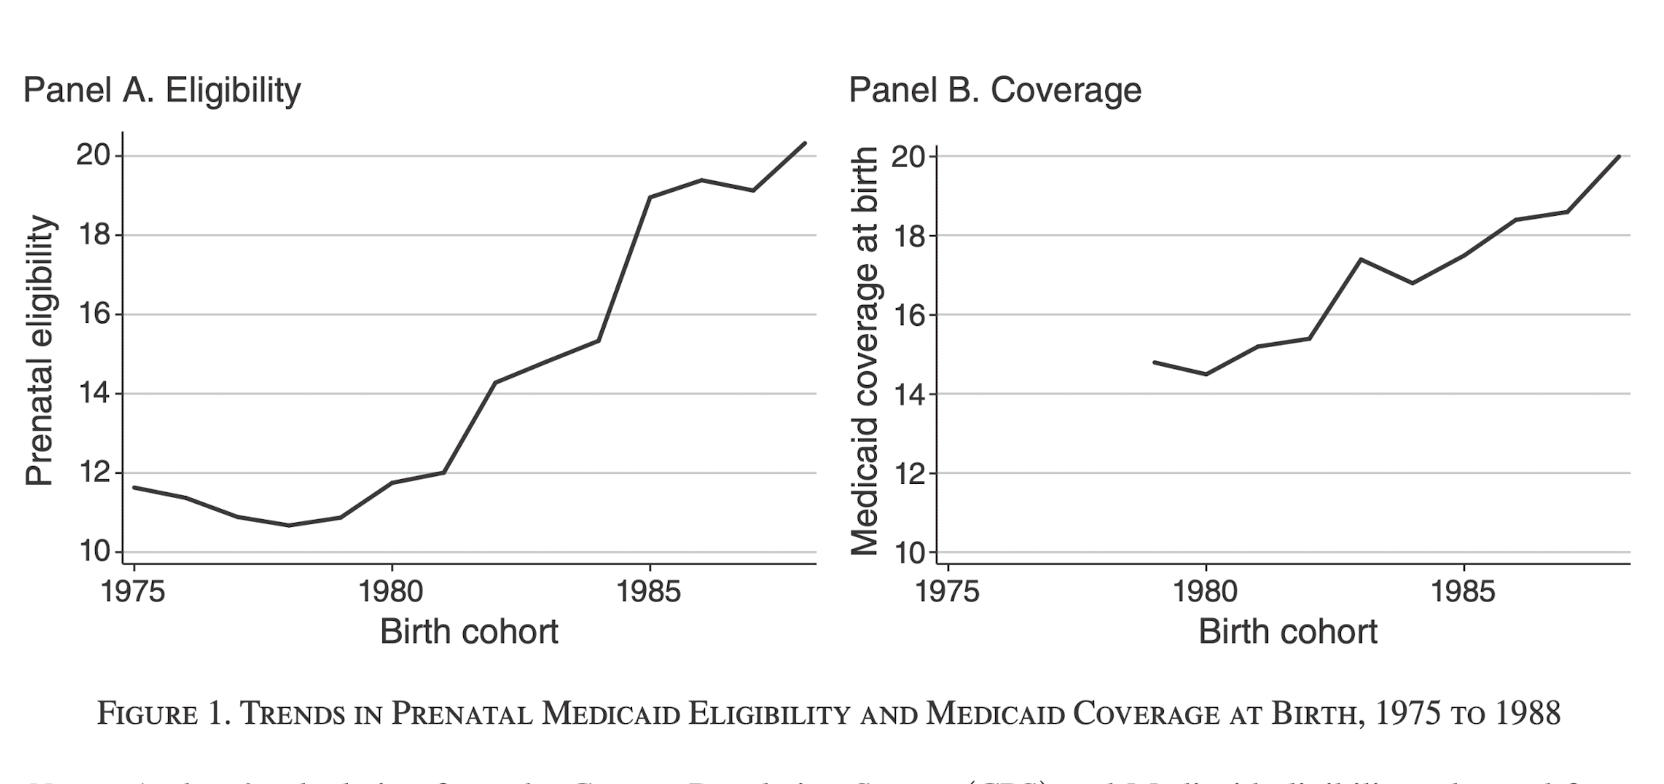
\includegraphics[height=0.8\textheight, width=\textwidth]{../Figures/fig_elig_birth.png}
\vspace{4pt}
\end{frame}

\begin{frame}{Targeted Prenatal Medicaid Expansions (1980–1985)}
\begin{itemize}
  \item States expanded eligibility for pregnant women at different times.
  \item Design uses \textbf{sharp eligibility jumps} (treated states) vs \textbf{no sharp jump} (controls).
  \item Key idea: compare cohorts born relative to each state's expansion year.
\end{itemize}
\end{frame}

\begin{frame}{Treated vs Control States}
\centering
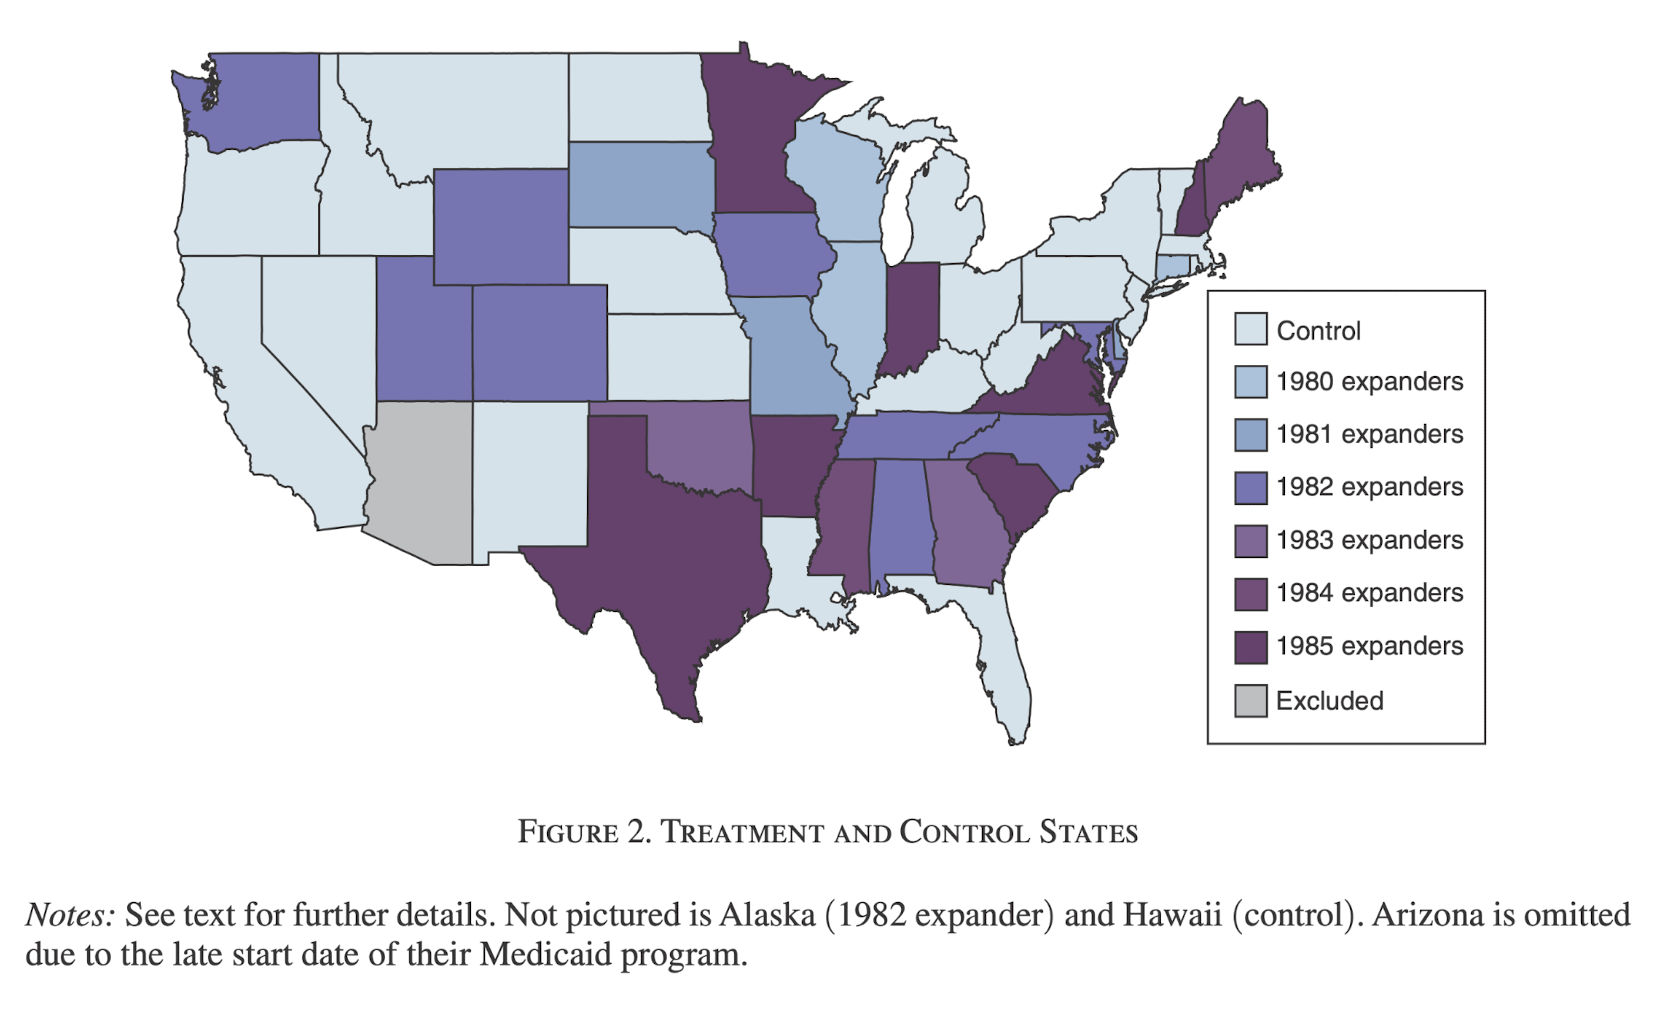
\includegraphics[height=0.78\textheight]{../Figures/fig_map_states.png}
\vspace{6pt}
\begin{itemize}
  \item Treated states: first large discrete eligibility jump in 1980–1985.
  \item Controls: no large discrete jump in the same window.
\end{itemize}
\end{frame}

\begin{frame}{Eligibility Trends}
\centering
  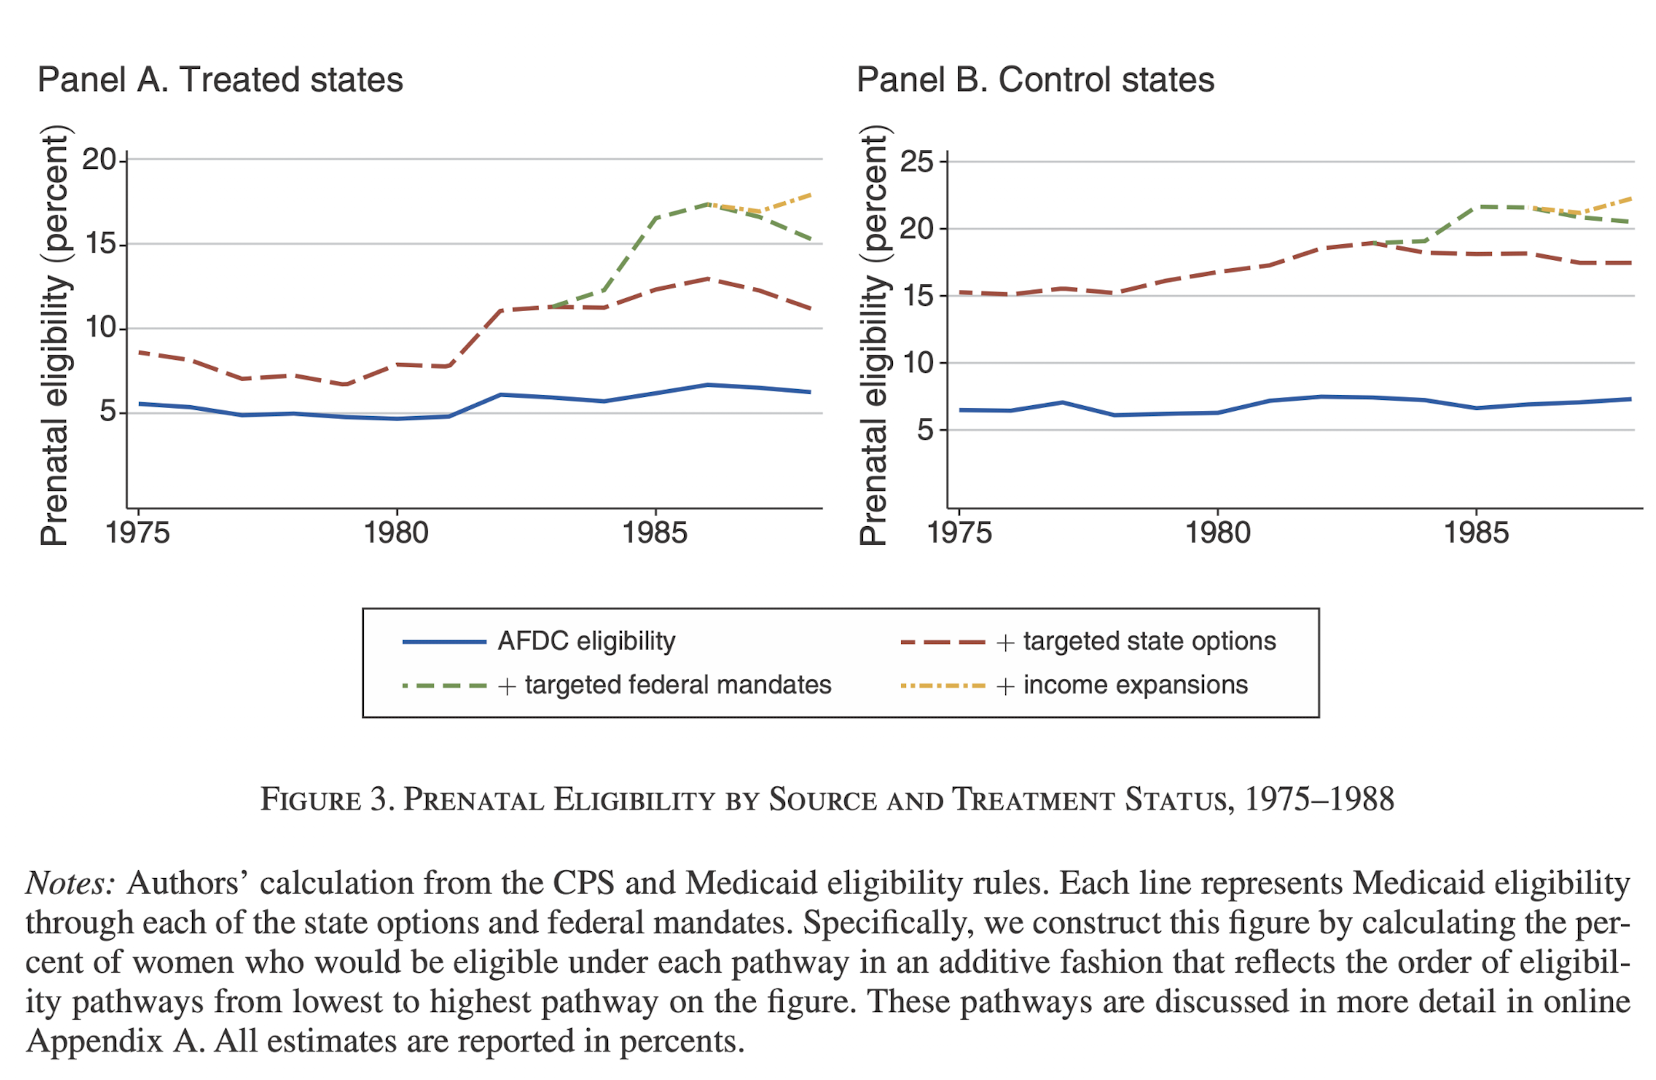
\includegraphics[height=0.78\textheight]{../Figures/fig_eligibility_trend.png}

\vspace{0.25cm}
\footnotesize Sources of eligibility growth: AFDC rules, targeted state options, targeted federal mandates, later income-based expansions.
\end{frame}

% -------------------------
\section{Empirical design}
% -------------------------

\begin{frame}{Event-Study Design}
\small
For cohorts born in state $n$ and year $b$:
\[
y_{nb} = \alpha + \sum_{t\in[-5,4] \setminus \{-1\}} \beta_t \, \mathbf{1}\{b - e_n = t\}
+ \eta_n + \lambda_b + \gamma X_{nb} + \varepsilon_{nb} .
\]
\begin{itemize}
  \item $e_n$: first year of the state's large eligibility jump.
  \item Omit $t=-1$ (year just before expansion): coefficients are relative to that baseline.
  \item Detrend using pre-period linear trend (state-specific), then estimate event study.
\end{itemize}
\end{frame}

\begin{frame}{Linking Treatment Across Generations}
\begin{itemize}
  \item \textbf{First generation}: outcomes of infants born 1975–1988; treatment assigned by \emph{state \& year of birth}.
  \item \textbf{Second generation}: infants born to first-generation mothers; treatment assigned by \emph{mother's state \& year of birth}.
  \item Vital Statistics birth records provide:
  \begin{itemize}
    \item infant outcomes
    \item mother characteristics including state of birth and (approx.) birth year.
  \end{itemize}
\end{itemize}
\end{frame}

\begin{frame}{Data}
\begin{itemize}
  \item \textbf{Vital Statistics natality data (1975–2017)}: universe of US births.
  \item \textbf{CPS ASEC + eligibility rules}: simulated prenatal eligibility.
  \item \textbf{NHDS hospital discharge data}: Medicaid coverage at delivery (first-stage validation).
  \begin{itemize}
    \item Accessed restricted variables via FRDC, like state of birth
  \end{itemize}
  \item \textbf{International Classification of Diseases}: labor and delivery hospitalization records (1979-1988) 
\end{itemize}
\end{frame}

\begin{frame}{Sample}
  \begin{itemize}
    \item First-Generation:
    \begin{enumerate}
      \item Born 1975-1988 (observe full cohort fertility through age 28)
    \end{enumerate}
    \item Second-Generation
    \begin{enumerate}
      \item First born to mother in a treated cohort
      \item Mother born in US (except Arizona)
      \item Born between 1990-2017
    \end{enumerate}
  \end{itemize}
\end{frame}

\begin{frame}{Methods: Mechanisms and Assumptions}
\begin{itemize}
  \item \textbf{Event time}: relative to each treated state's \emph{first large discrete} eligibility jump.
  \item \textbf{Detrending}: remove state-specific linear pretrends (estimated on the preperiod).
  \item \textbf{Controls}: state-year covariates (economy, welfare policy, abortion policy) + demographic controls.
  \item \textbf{Weighting}: by cohort size (population-weighted estimates).
  \item \textbf{Inference}: clustered SEs at the state level (state of birth / mother's state of birth).
\end{itemize}
\end{frame}

\begin{frame}{Threats to Identification and Overcoming Them}
\begin{itemize}
  \item \textbf{Endogenous expansion timing}: pretrend diagnostics + detrending; robustness to alternative FE/control sets.
  \item \textbf{Other policy/economic changes}: state-year controls; robustness checks (e.g., add region-year FE, drop control states).
  \item \textbf{Composition (fertility/migration) changes}: sensitivity to weighting and sample restrictions.
  \item \textbf{Confounding from later childhood Medicaid expansions}: add later-eligibility measures; patterns remain similar.
  \item \textbf{Treatment assignment error (2nd gen)}: use mother's state/year of birth; stability across specs.
\end{itemize}
\end{frame}

% -------------------------
\section{First Stage and Validation}
% -------------------------


\begin{frame}{Actual vs. Simulated Eligibility}
  \centering
  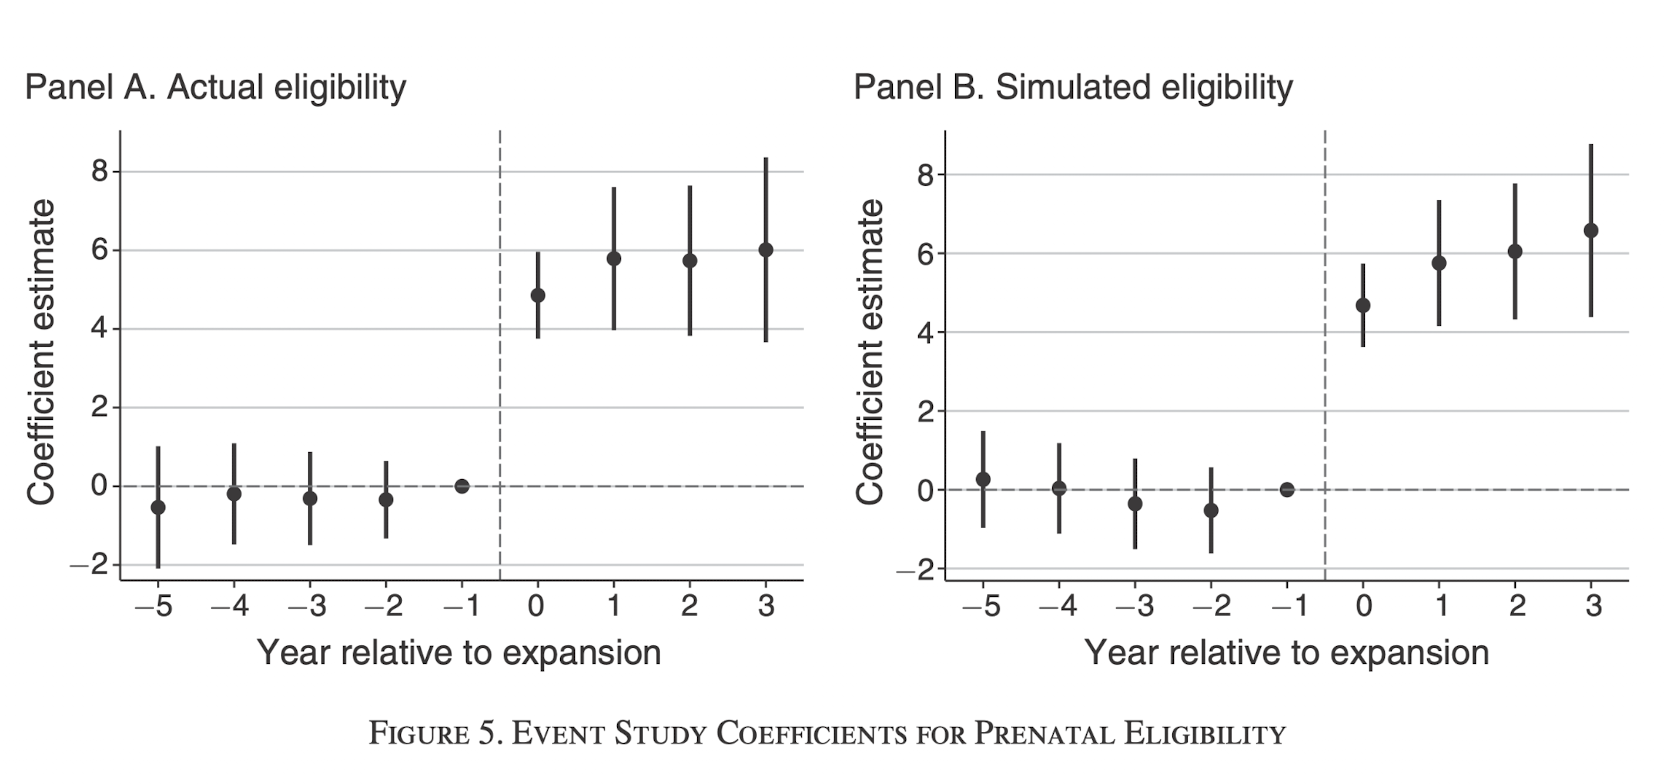
\includegraphics[height=0.78\textheight, width=\textwidth]{../Figures/fig_first_elig.png}
\end{frame}

% -------------------------
\section{Main Results}
% -------------------------


\begin{frame}{First-Generation: Low Birth Weight Declines}
\centering
  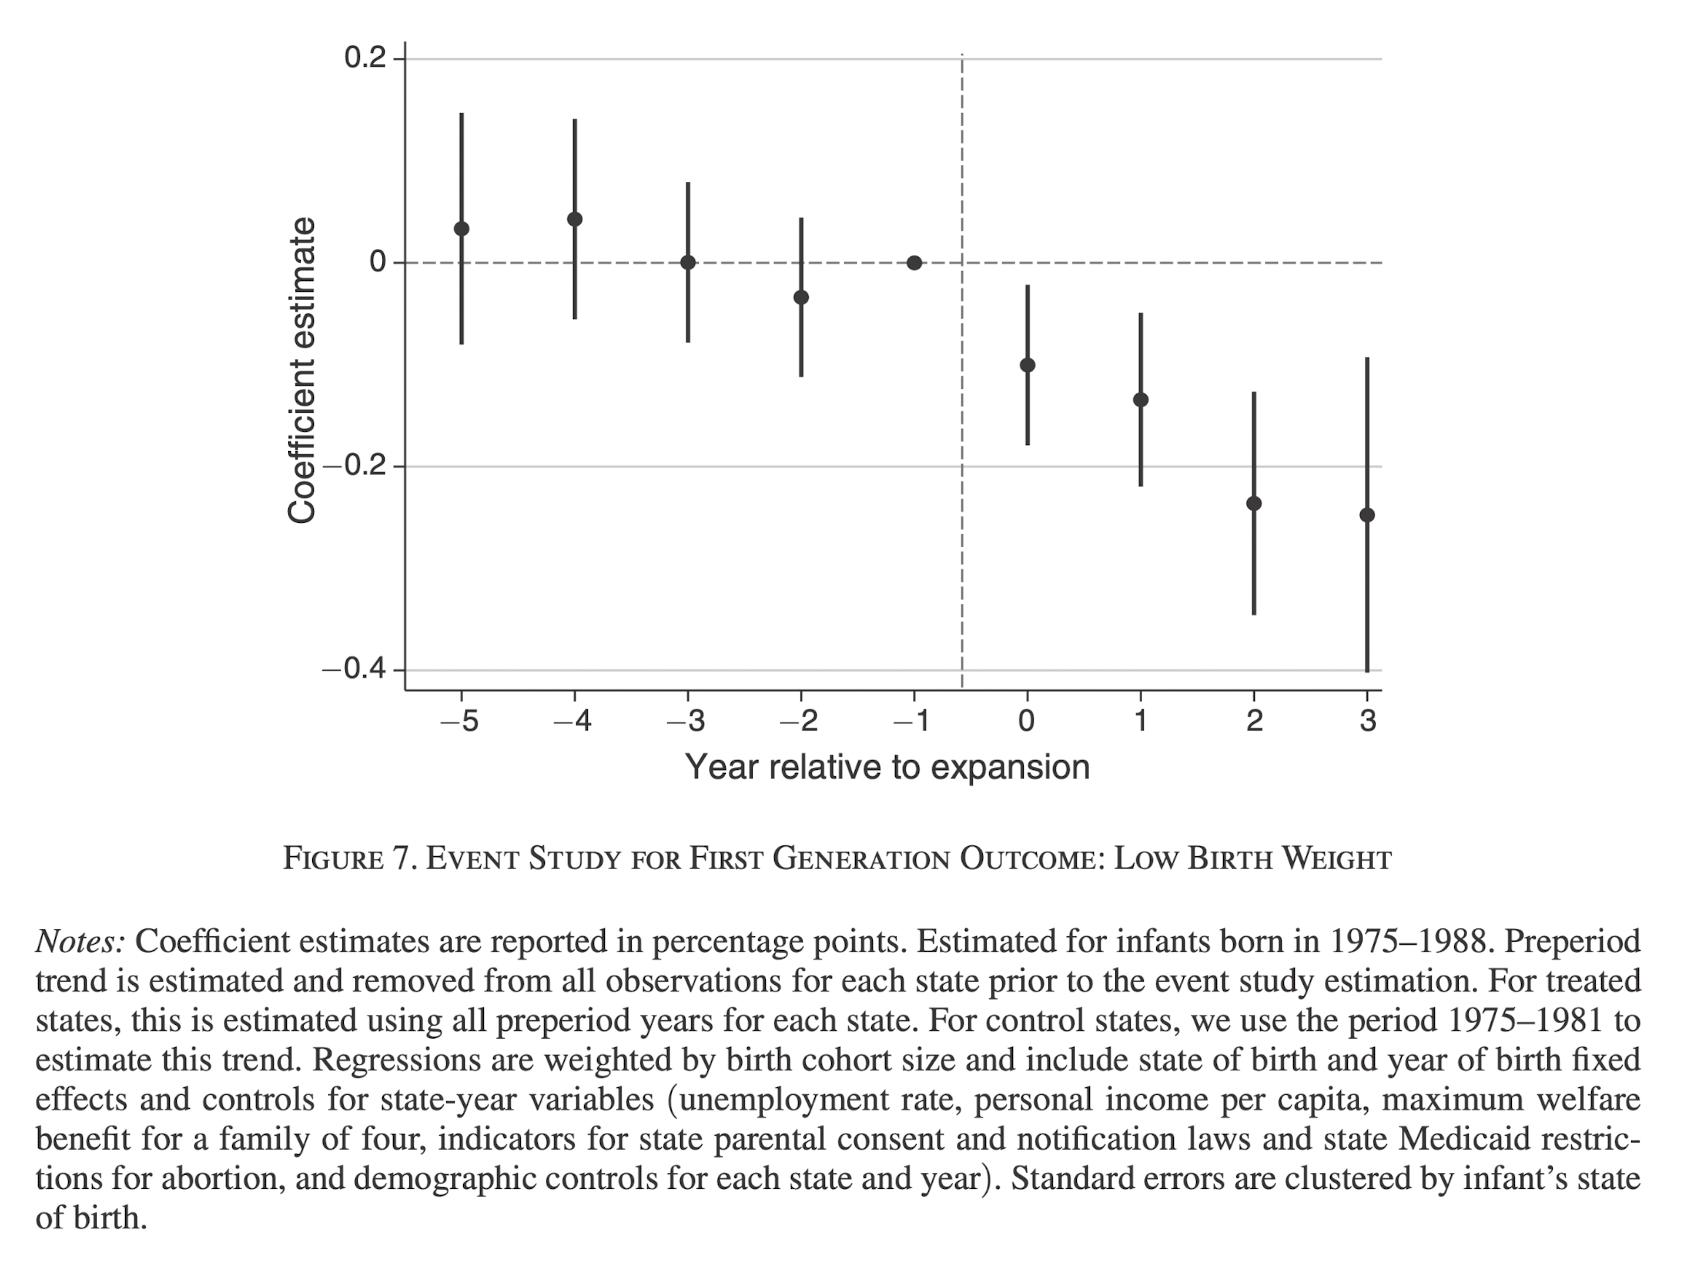
\includegraphics[heigh=0.78\textwidth, width=\textwidth]{../Figures/fig_first_lbw.png}
\vspace{4pt}
\end{frame}

\begin{frame}{Second-Generation: Birth Weight Improves}
\centering
  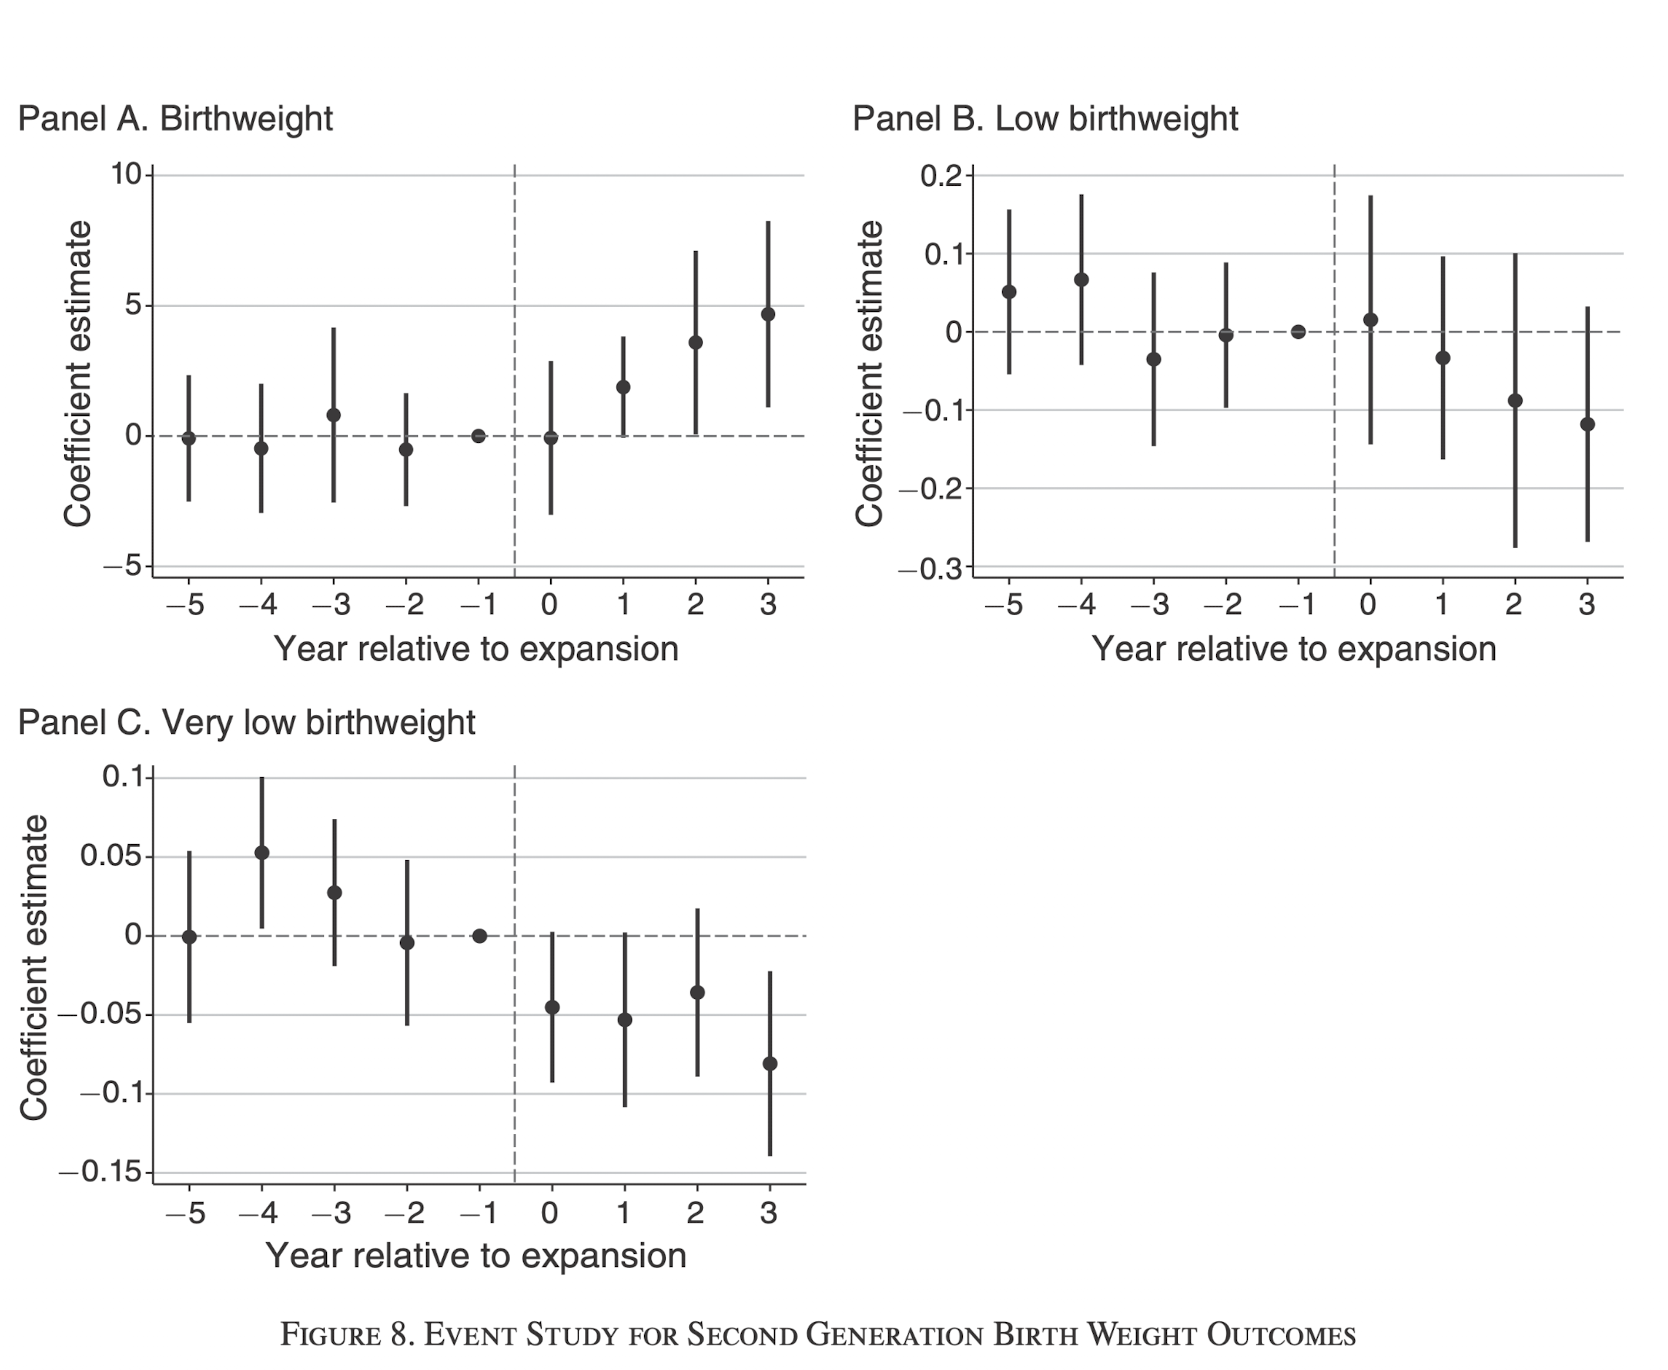
\includegraphics[height=.99\textheight, width=\textwidth]{../Figures/fig_second_lbw.png}
\vspace{4pt}
\end{frame}

\begin{frame}{Second-Generation: Gestational Outcomes}
\centering
  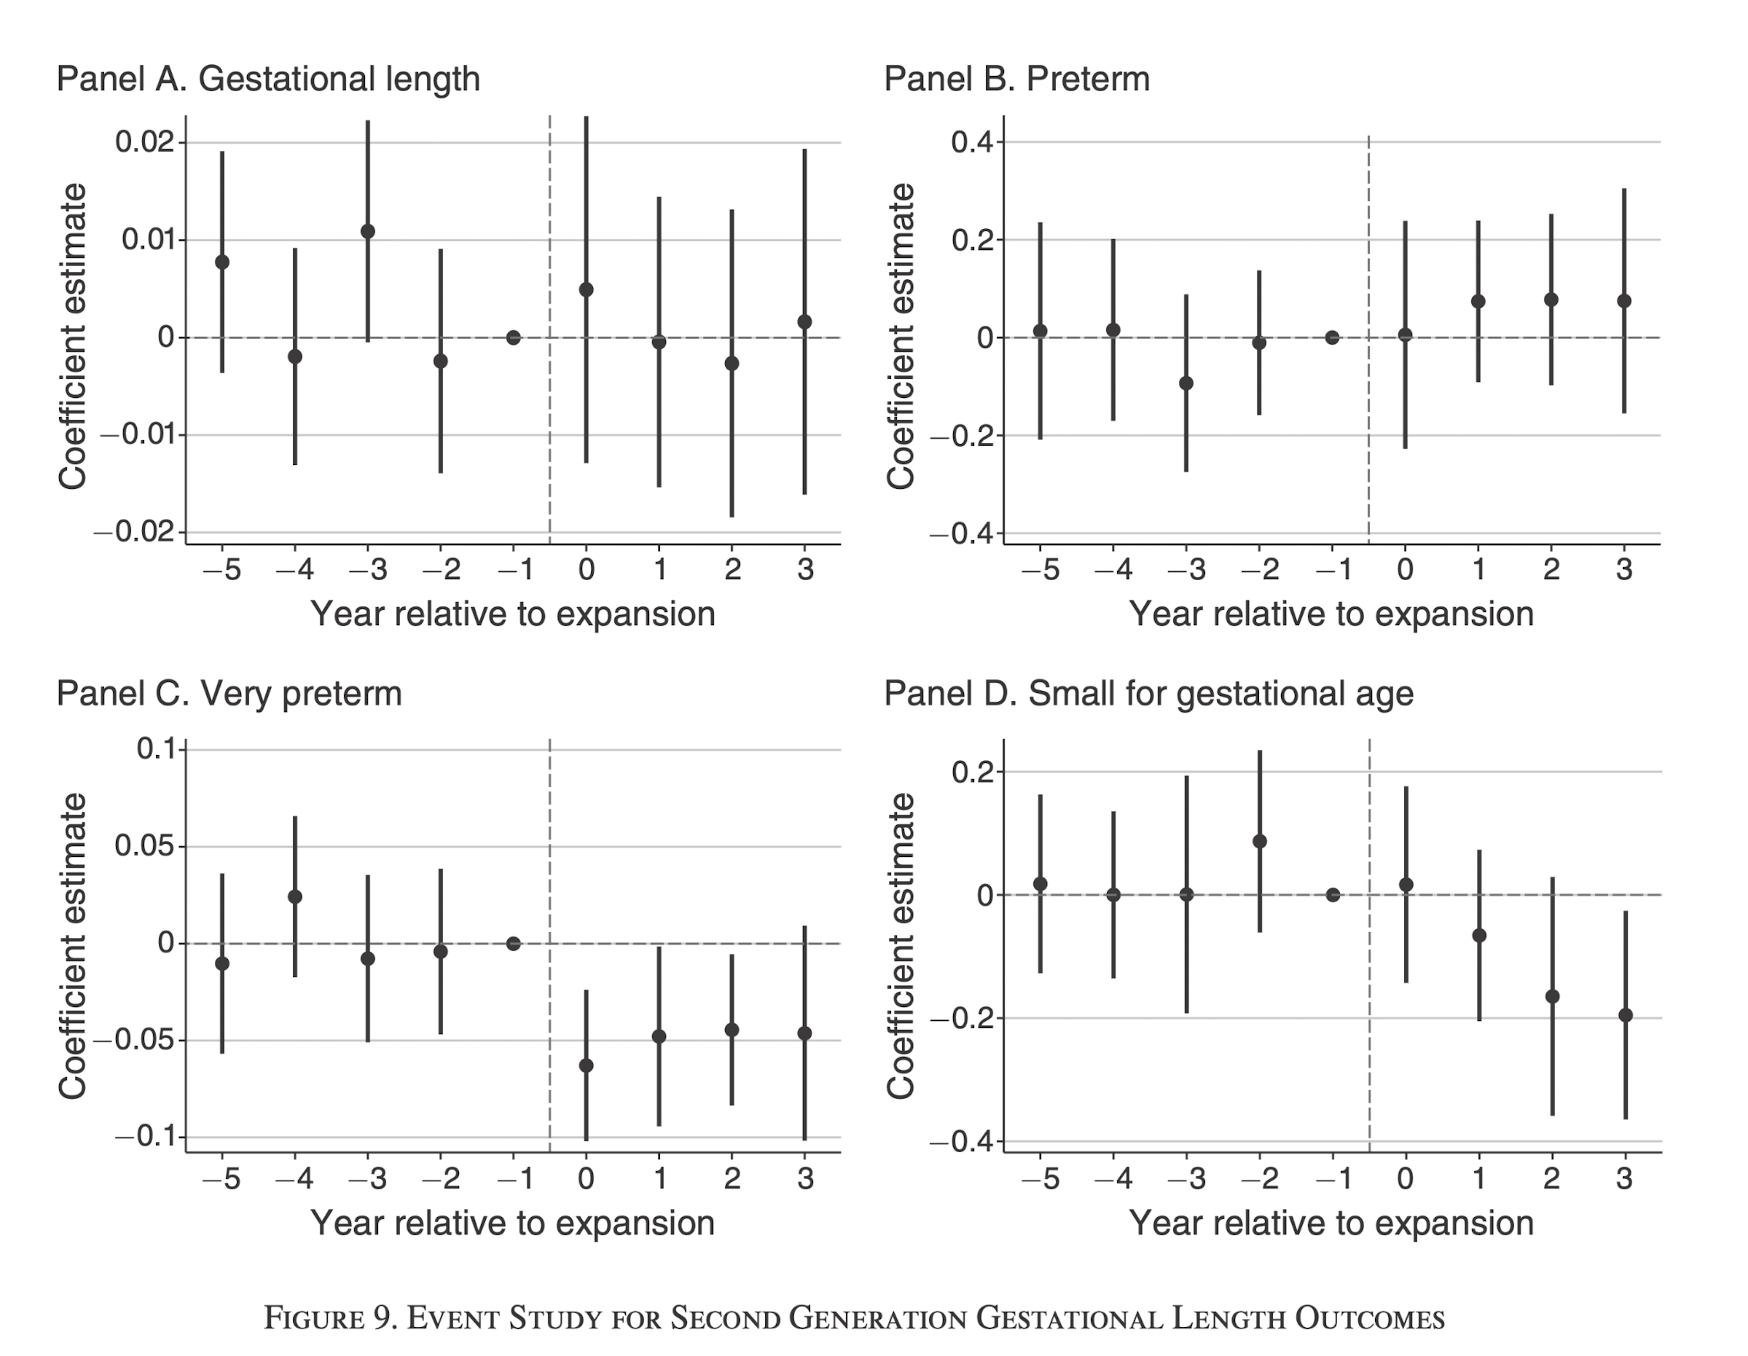
\includegraphics[height=0.99\textheight, width=\textwidth]{../Figures/fig_second_gest.png}
\end{frame}

\begin{frame}{Robustness: Alternative Controls and Specifications}
\centering
  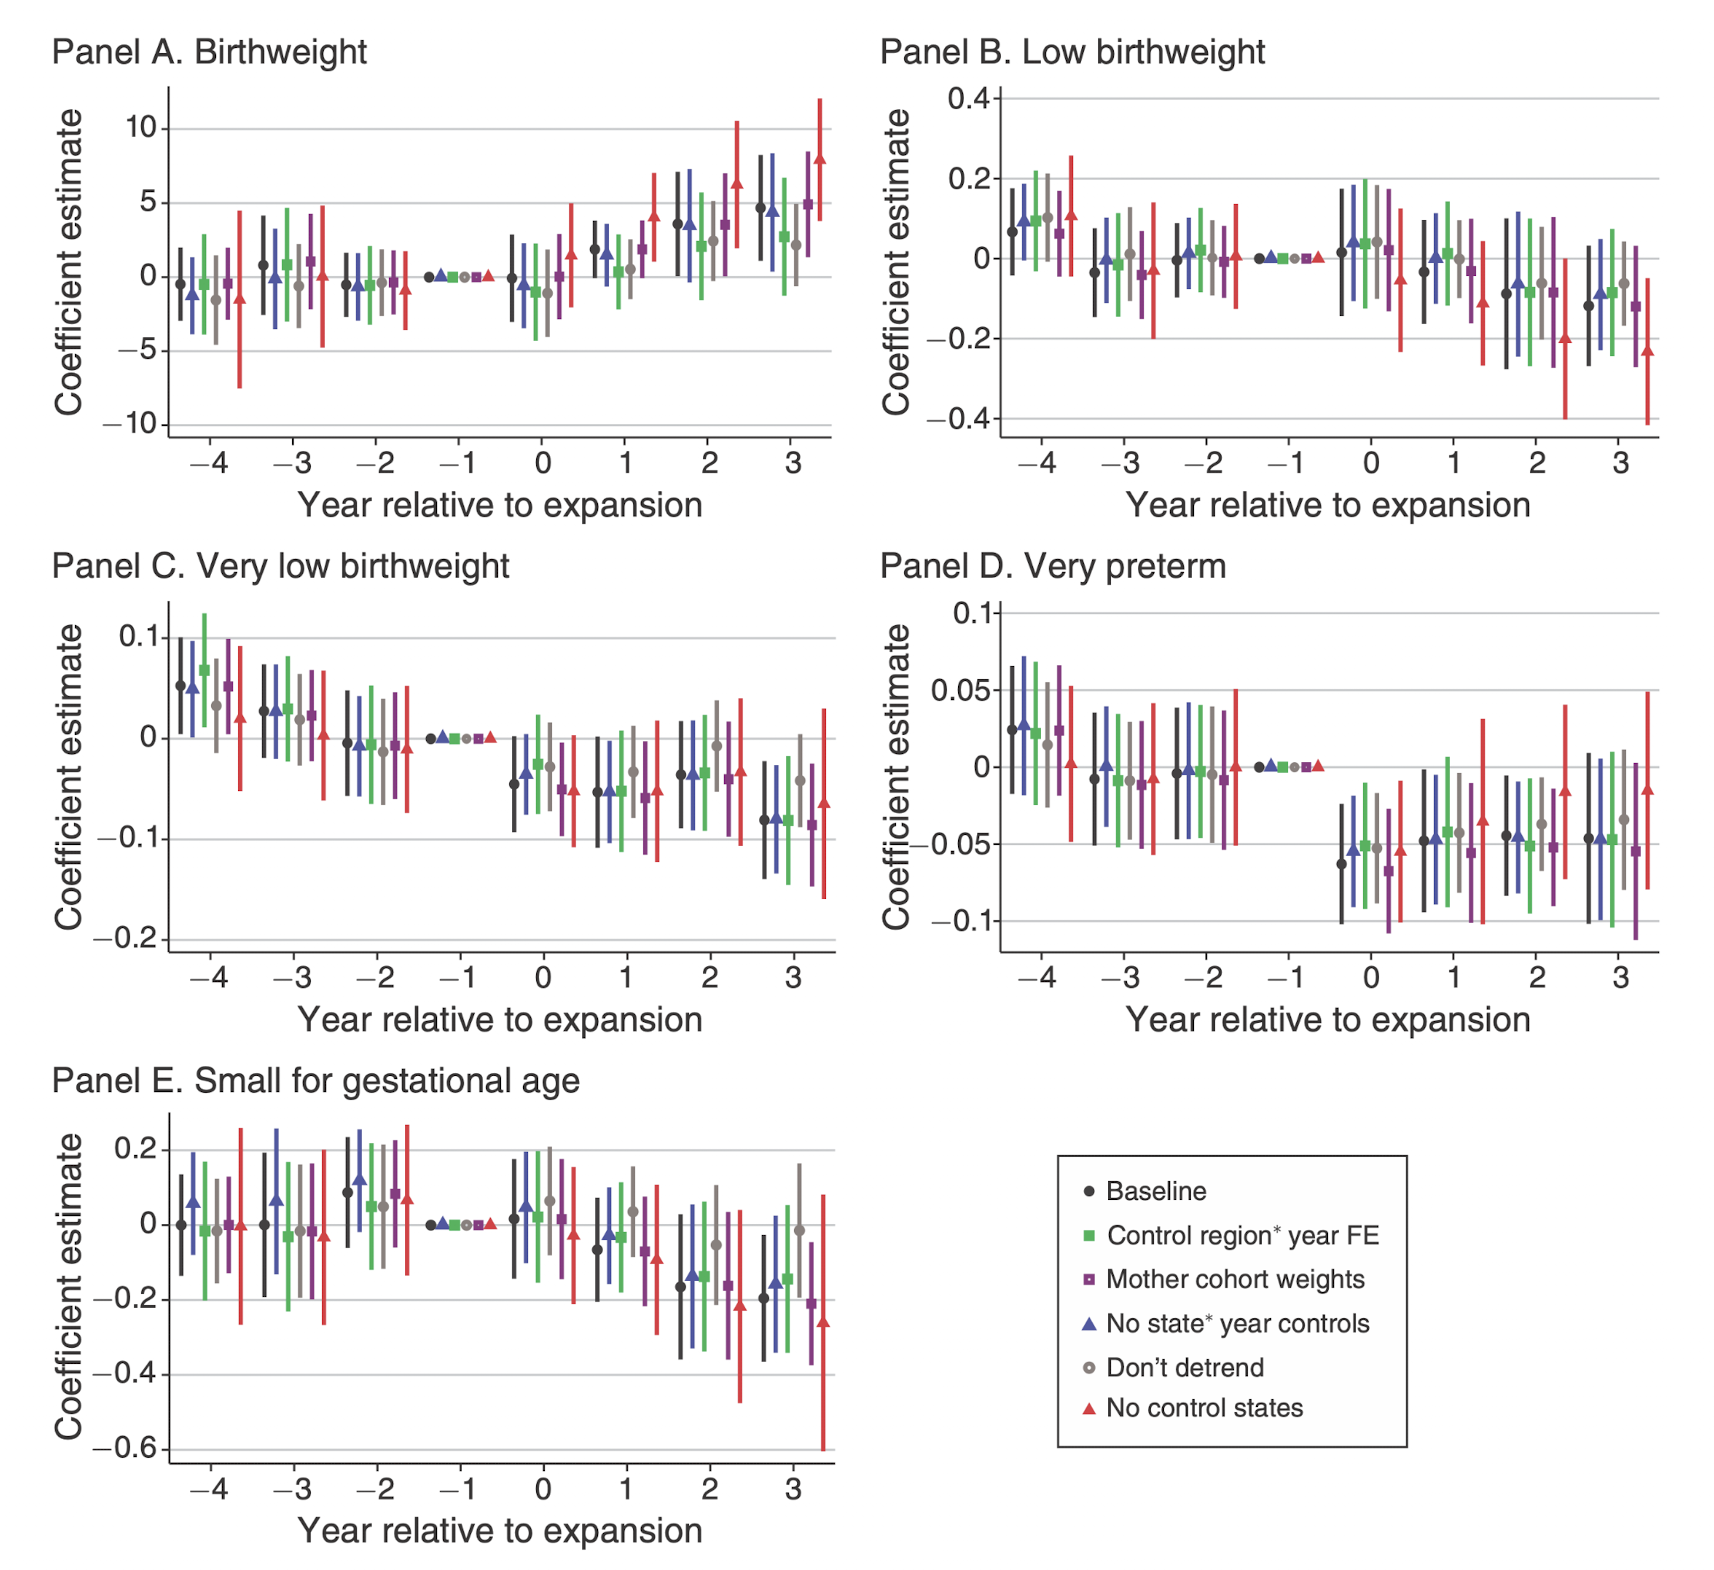
\includegraphics[height=0.9\textheight, width=\textwidth]{../Figures/fig_robustness.png}
\end{frame}

% -------------------------
\section{Interpretation}
% -------------------------

\begin{frame}{Mechanisms}
\begin{itemize}
  \item Biological pathway: improved maternal health endowments at birth
  \item Maternal health during pregnancy: lower chronic disease risk, better prenatal environment
  \item Non-biological channels: stress reduction, resources, and prenatal care
\end{itemize}
\end{frame}

\begin{frame}{Policy Interpretation}
\begin{itemize}
  \item Multigenerational benefits imply standard program evaluations may understate returns
  \item Medicaid expansions are not only safety-net insurance:
  \begin{itemize}
    \item they change early-life health trajectories, which lead to improved later-life circumstances
    \item and those changes can transmit to the next generation
  \end{itemize}
\end{itemize}
\end{frame}

% -------------------------
\section{Conclusion}
% -------------------------

\begin{frame}{Takeaways}
\begin{itemize}
  \item Prenatal Medicaid expansions improved first-generation infant health, in line with past results
  \item Those improvements transmit: second-generation birth outcomes also improve, though to a lesser degree
  \item Implementation of policy should keep the potential spillovers in mind, as the initial payoff could essentially be thought of as investment into future outcomes 
\end{itemize}
\end{frame}

\end{document}
